%!TEX root = ./main.tex
\section{Overview}
\label{sec2}

In this section, we show a simple example processed by existing approach and our approach. Firstly, we define a simple core language with following syntax and semantic.
\[
\begin{array}{lll}
\m{e} &::=& \Code{(if~e~e~e)}\\
& |& \true\\
& |& \false
\end{array}
\]

\infrule[context rule of if]
{\m{e}~\rightarrow~\m{e'}}
{\Code{(if e e1 e2)}\rightarrow\Code{(if e' e1 e2)}}
\infax[reduction rule of iftrue]
{\Code{(if \#t e1 e2)}\rightarrow \m{e1}}
\infax[reduction rule of iffalse]
{\Code{(if \#f e1 e2)} \rightarrow \m{e2}}

We define two syntactic sugars---\emph{and} sugar and \emph{or} sugar based on the core language.

\[
\drule{\Code{(and e1 e2)}}{\Code{(if e1 e2 \#f)}}
\]
\[
\drule{\Code{(or e1 e2)}}{\Code{(if e1 \#t e2)}}
\]
and execute \Code{(and (or \#t \#f) (and \#f \#t))} as an example.

\subsection{Existing resugaring approach}
As we mentioned above, the existing approach use "tagging" and "reverse desugaring" to get resugaring sequences. Tags is to show where are terms from, and reverse dusugaring is what resugaring needs. We simplify the existing resugaring process as follows.

\begin{Codes}
    (and (or \#t \#f) (and \#f \#t))
\DeStep{  (if-andtag (if-ortag \#t \#t \#f) (if-andtag \#f \#t \#f) \#f)}  \note{//desugar}
\note{ start evaluating}  
\OneStep{ (if-andtag \#t (if-andtag \#f \#t \#f) \#f)} \note{//check resugarable}
\note{ get (and \#t (and \#f \#t)) by reverse desugaring}
\OneStep{ (if-andtag \#f \#t \#f)} \note{//check resugarable}
\note{ get (and \#f \#t) by reverse desugaring}
\OneStep{ #f} \note{end of resugaring}
\end{Codes}

We can find that the expression fully desugared before resugaring. The subexpression \Code{(and \#f \#t)}, though desugars to \Code{(if-andtag \#f \#t \#f)}, doesn't be reduced in first two steps after desugaring. But the reverse desugaring tries on it in these two steps, which is redundant. Moreover, there will be some intermediate steps which can not be resugared by reverse desugaring during the evaluation in a more complex core language. Many useless resugarings on subexpressions will take place.

%Use a simple but sharp example to give an overview of your approach.
\subsection{Resugaring by lazy desugaring}

\ignore{
    \begin{figure}[t]
    \centering
    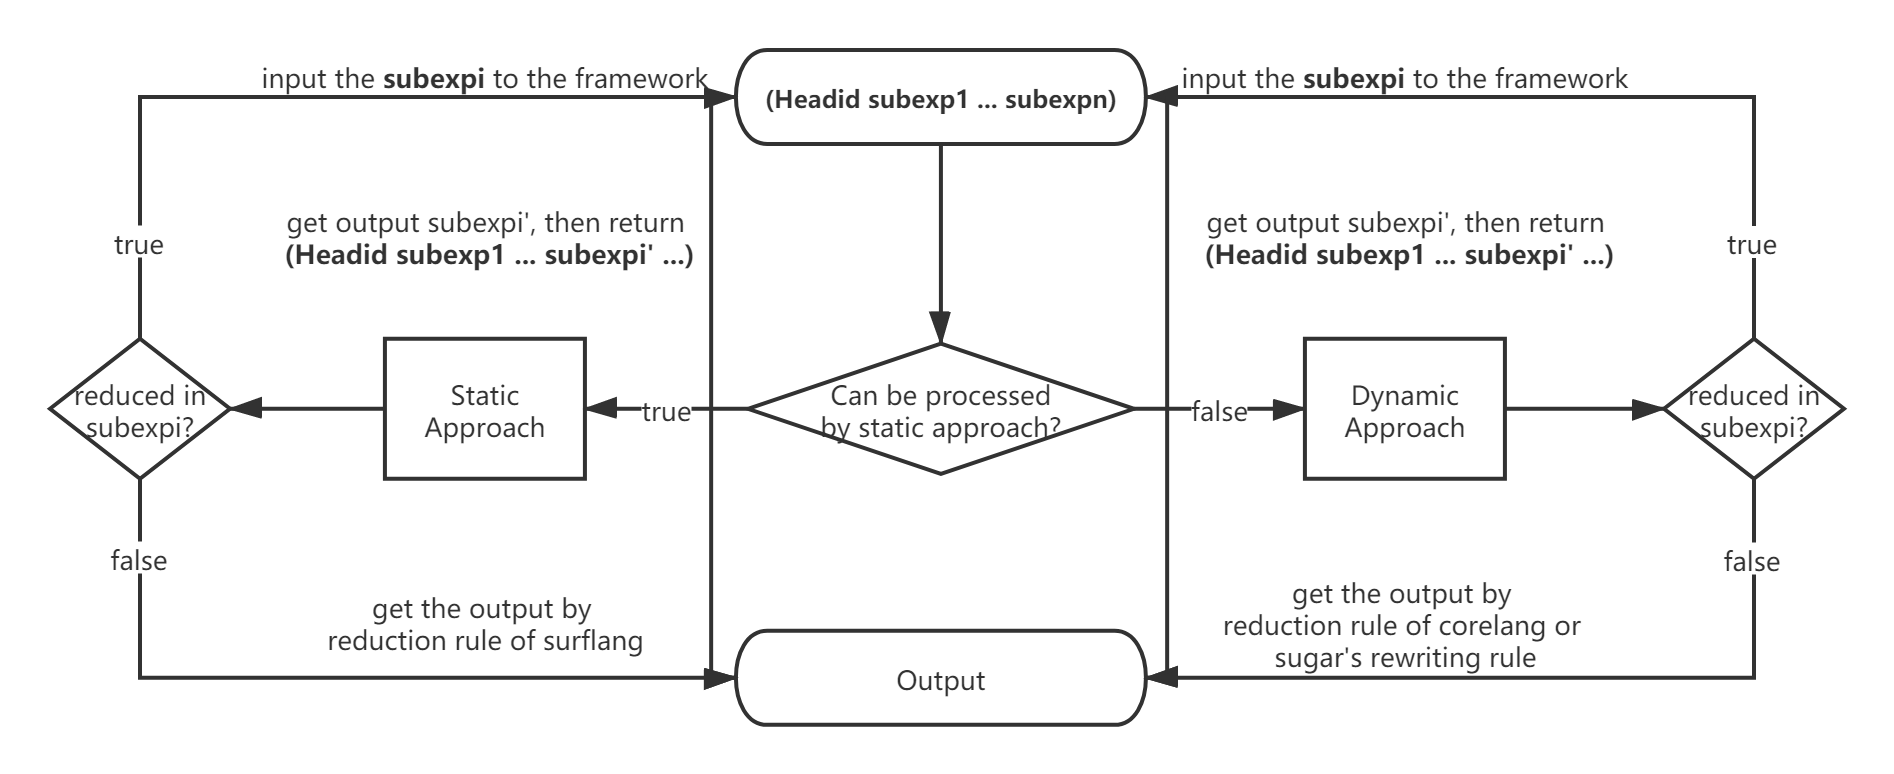
\includegraphics[width=12cm]{images/mixture.png}
    \caption{One step in framework of mixture approach}
    \label{fig:mixture}
\end{figure}

Given an example based on the former section. Besides sugar {\bfseries and}, {\bfseries or}, we add a recursive sugar {\bfseries mapf} based on another new sugar {\bfseries f}. The recursive sugar can be handled by the dynamic approach, but not for the static one. (Reasons in later sections)
\begin{Codes}
\small{(f e1 e2)} \DeStep{ (let x e1 (or x (and e2 x)))}
\small{(mapf e lst)} \DeStep{ (if (empty? lst) empty (cons (f e (first lst)) (mapf e (rest lst))))}
\end{Codes}

In the mapf (map of f) sugar, we use both core language's term (such as {\bfseries if, empty?, cons, let, first, rest}) and existing syntactic sugar ({\bfseries and, or}). The semantics of core language is as common. But to show some exact steps, we set the term {\bfseries cons} as a common expression (belonging to core language, but being displayed as surface language).


If we execute
\begin{Codes}
(mapf \#t (list \#f \#t))
\end{Codes}
 the mixture approach will judge whether sugar mapf can be handle by the static approach. No, then we use the dynamic approach in one step and get the intermediate expression.
\begin{Codes}
    (mapf \#t (list \#f \#t))
\OneStep{ (cons (f \#t (first (list \#f \#t))) (mapf \#t (rest (list \#f \#t))))}
\end{Codes}
Then according to semantics of {\bfseries cons}, the first subexpression should be reduced. The subexpression can be handled by the static approach, so getting a subsequence.
\begin{Codes}
    (cons (f \#t (first (list \#f \#t))) (mapf \#t (rest (list \#f \#t))))
\OneStep{ (cons (f \#t \#f) (mapf \#t (rest (list \#f \#t))))}
\OneStep{ (cons \#t (mapf \#t (rest (list \#f \#t))))}
\end{Codes}
Then the second subexpression should be reduced, which is a recursive process. Finally, the subexpression (mapf \#t (list)) will be processed by dynamic approach.
\begin{Codes}
   (mapf \#t (list))
\DeStep{ (if (empty? (list)) empty ...)}
\OneStep{ empty}
\end{Codes}
Note that there are some steps should not be displayed, we define the common expressions above in syntaxes to restrict which intermediate step should be displayed.
}

To solve the problem in existing resugaring approach, we try "lazy desugaring", which means that a syntactic sugar should only desugar when it has to desugar. We use a one-step try method to judge it.
\begin{Codes}
    (resugar (and (or \#t \#f) (and \#f \#t)))
\DeStep{  (tmp (if (or \#t \#f) (and \#f \#t) \#f))} \note{// should reduce on (or \#t \#f)}
\OneStep{ (and (resugar (or \#t \#f)) (and \#f \#t))} \note{// no reduction}
\DeStep{  (and (tmp (if \#t \#t \#f)) (and \#f \#t))} \note{//  (or \#t \#f) has to desugar and reduce}
\OneStep{ (desugar (and \#t (and \#f \#t)))}
\DeStep{  (tmp (if \#t (and \#f \#t)))} \note{// the outermost \emph{and} sugar has to desugar and reduce}
\OneStep{ (desugar (and \#f \#t))}
\DeStep{  (tmp (if \#f \#t \#f))} \note{// have to desugar and reduce}
\OneStep{ \#f} \note{// end}
\end{Codes} 

For each step in the processes above we use one reduction or none. So 7 reduction steps is needed for the whole resugaring, while the existing approach needs 9 (3 in desugaring, 3 in evaluator, 3 reversed reduction in resugaring). Note that reversed reduction is more complex because of the match and substitution, the existing approach will be more redundant on larger expressions than ours. Also, there is no need for tagging, which makes our approach lightweight.

Moreover, derivation of semantics for syntactic sugar will make our approach more efficient for part of sugars. Both \emph{and} sugar and \emph{or} sugar can be handled by the derivation. We can get the following semantics (consisted of reduction rules and context rules).
\[
\begin{array}{c}
\infer {(\mbox{and}~e_1~e_2) \rightarrow (\mbox{and}~e_1'~e_2)} {e_1~ \rightarrow~e_1'}\\
(\mbox{and}~\#t~e2) \rightarrow e_2 \\
(\mbox{and}~\#f~e2) \rightarrow \#f \\
\infer {(\mbox{or}~e_1~e_2) \rightarrow (\mbox{or}~e_1'~e_2)} {e_1~ \rightarrow~e_1'}\\
(\mbox{or}~\#t~e2) \rightarrow \#t \\
(\mbox{or}~\#f~e2) \rightarrow e_2 \\
\end{array}
\]
Then the resugaring sequences can be got not depending on core language.
\begin{Codes}
    (and (or \#t \#f) (and \#f \#t))
\OneStep{ (and \#t (and \#f \#t))}
\OneStep{ (and \#f \#t)}
\OneStep{ \#f}
\end{Codes}

Only 4 steps is needed by using the rules. Although the derivation of rules cannot work for all syntactic sugars which can be handled by our resugaring approach, it can work together with the resugaring. For example, we have another sugar named \emph{hard} (regardless of its desugar rule) whose reduction rules cannot be derivate.
Then if we execute \Code{(and (hard (and \#t \#t) ...) ...)}, the \emph{and}'s semantics will let the \emph{hard} sugar execute recursively. Then the sugar \emph{hard} will be processed by our basic resugaring approach because no semantic rules for it. Note that the resugaring process may also recursively execute on inner subexpression (e.g. \Code{(and \#t \#t)}), the subexpression may use the semantic rules again.

In summary, our resugaring approach with lazy desugaring is lightweight and efficient. Following chapters will show that, though lightweight, the approach is more powerful than existing approach in some ways.
\todo{following chapter will also show lightweight and efficient. but how to express?}